% Options for packages loaded elsewhere
\PassOptionsToPackage{unicode}{hyperref}
\PassOptionsToPackage{hyphens}{url}
\PassOptionsToPackage{dvipsnames,svgnames,x11names}{xcolor}
%
\documentclass[
  letterpaper,
  DIV=11,
  numbers=noendperiod]{scrartcl}

\usepackage{amsmath,amssymb}
\usepackage{lmodern}
\usepackage{iftex}
\ifPDFTeX
  \usepackage[T1]{fontenc}
  \usepackage[utf8]{inputenc}
  \usepackage{textcomp} % provide euro and other symbols
\else % if luatex or xetex
  \usepackage{unicode-math}
  \defaultfontfeatures{Scale=MatchLowercase}
  \defaultfontfeatures[\rmfamily]{Ligatures=TeX,Scale=1}
\fi
% Use upquote if available, for straight quotes in verbatim environments
\IfFileExists{upquote.sty}{\usepackage{upquote}}{}
\IfFileExists{microtype.sty}{% use microtype if available
  \usepackage[]{microtype}
  \UseMicrotypeSet[protrusion]{basicmath} % disable protrusion for tt fonts
}{}
\makeatletter
\@ifundefined{KOMAClassName}{% if non-KOMA class
  \IfFileExists{parskip.sty}{%
    \usepackage{parskip}
  }{% else
    \setlength{\parindent}{0pt}
    \setlength{\parskip}{6pt plus 2pt minus 1pt}}
}{% if KOMA class
  \KOMAoptions{parskip=half}}
\makeatother
\usepackage{xcolor}
\usepackage[normalem]{ulem}
\setlength{\emergencystretch}{3em} % prevent overfull lines
\setcounter{secnumdepth}{5}
% Make \paragraph and \subparagraph free-standing
\ifx\paragraph\undefined\else
  \let\oldparagraph\paragraph
  \renewcommand{\paragraph}[1]{\oldparagraph{#1}\mbox{}}
\fi
\ifx\subparagraph\undefined\else
  \let\oldsubparagraph\subparagraph
  \renewcommand{\subparagraph}[1]{\oldsubparagraph{#1}\mbox{}}
\fi

\usepackage{color}
\usepackage{fancyvrb}
\newcommand{\VerbBar}{|}
\newcommand{\VERB}{\Verb[commandchars=\\\{\}]}
\DefineVerbatimEnvironment{Highlighting}{Verbatim}{commandchars=\\\{\}}
% Add ',fontsize=\small' for more characters per line
\usepackage{framed}
\definecolor{shadecolor}{RGB}{241,243,245}
\newenvironment{Shaded}{\begin{snugshade}}{\end{snugshade}}
\newcommand{\AlertTok}[1]{\textcolor[rgb]{0.68,0.00,0.00}{#1}}
\newcommand{\AnnotationTok}[1]{\textcolor[rgb]{0.37,0.37,0.37}{#1}}
\newcommand{\AttributeTok}[1]{\textcolor[rgb]{0.40,0.45,0.13}{#1}}
\newcommand{\BaseNTok}[1]{\textcolor[rgb]{0.68,0.00,0.00}{#1}}
\newcommand{\BuiltInTok}[1]{\textcolor[rgb]{0.00,0.23,0.31}{#1}}
\newcommand{\CharTok}[1]{\textcolor[rgb]{0.13,0.47,0.30}{#1}}
\newcommand{\CommentTok}[1]{\textcolor[rgb]{0.37,0.37,0.37}{#1}}
\newcommand{\CommentVarTok}[1]{\textcolor[rgb]{0.37,0.37,0.37}{\textit{#1}}}
\newcommand{\ConstantTok}[1]{\textcolor[rgb]{0.56,0.35,0.01}{#1}}
\newcommand{\ControlFlowTok}[1]{\textcolor[rgb]{0.00,0.23,0.31}{#1}}
\newcommand{\DataTypeTok}[1]{\textcolor[rgb]{0.68,0.00,0.00}{#1}}
\newcommand{\DecValTok}[1]{\textcolor[rgb]{0.68,0.00,0.00}{#1}}
\newcommand{\DocumentationTok}[1]{\textcolor[rgb]{0.37,0.37,0.37}{\textit{#1}}}
\newcommand{\ErrorTok}[1]{\textcolor[rgb]{0.68,0.00,0.00}{#1}}
\newcommand{\ExtensionTok}[1]{\textcolor[rgb]{0.00,0.23,0.31}{#1}}
\newcommand{\FloatTok}[1]{\textcolor[rgb]{0.68,0.00,0.00}{#1}}
\newcommand{\FunctionTok}[1]{\textcolor[rgb]{0.28,0.35,0.67}{#1}}
\newcommand{\ImportTok}[1]{\textcolor[rgb]{0.00,0.46,0.62}{#1}}
\newcommand{\InformationTok}[1]{\textcolor[rgb]{0.37,0.37,0.37}{#1}}
\newcommand{\KeywordTok}[1]{\textcolor[rgb]{0.00,0.23,0.31}{#1}}
\newcommand{\NormalTok}[1]{\textcolor[rgb]{0.00,0.23,0.31}{#1}}
\newcommand{\OperatorTok}[1]{\textcolor[rgb]{0.37,0.37,0.37}{#1}}
\newcommand{\OtherTok}[1]{\textcolor[rgb]{0.00,0.23,0.31}{#1}}
\newcommand{\PreprocessorTok}[1]{\textcolor[rgb]{0.68,0.00,0.00}{#1}}
\newcommand{\RegionMarkerTok}[1]{\textcolor[rgb]{0.00,0.23,0.31}{#1}}
\newcommand{\SpecialCharTok}[1]{\textcolor[rgb]{0.37,0.37,0.37}{#1}}
\newcommand{\SpecialStringTok}[1]{\textcolor[rgb]{0.13,0.47,0.30}{#1}}
\newcommand{\StringTok}[1]{\textcolor[rgb]{0.13,0.47,0.30}{#1}}
\newcommand{\VariableTok}[1]{\textcolor[rgb]{0.07,0.07,0.07}{#1}}
\newcommand{\VerbatimStringTok}[1]{\textcolor[rgb]{0.13,0.47,0.30}{#1}}
\newcommand{\WarningTok}[1]{\textcolor[rgb]{0.37,0.37,0.37}{\textit{#1}}}

\providecommand{\tightlist}{%
  \setlength{\itemsep}{0pt}\setlength{\parskip}{0pt}}\usepackage{longtable,booktabs,array}
\usepackage{calc} % for calculating minipage widths
% Correct order of tables after \paragraph or \subparagraph
\usepackage{etoolbox}
\makeatletter
\patchcmd\longtable{\par}{\if@noskipsec\mbox{}\fi\par}{}{}
\makeatother
% Allow footnotes in longtable head/foot
\IfFileExists{footnotehyper.sty}{\usepackage{footnotehyper}}{\usepackage{footnote}}
\makesavenoteenv{longtable}
\usepackage{graphicx}
\makeatletter
\def\maxwidth{\ifdim\Gin@nat@width>\linewidth\linewidth\else\Gin@nat@width\fi}
\def\maxheight{\ifdim\Gin@nat@height>\textheight\textheight\else\Gin@nat@height\fi}
\makeatother
% Scale images if necessary, so that they will not overflow the page
% margins by default, and it is still possible to overwrite the defaults
% using explicit options in \includegraphics[width, height, ...]{}
\setkeys{Gin}{width=\maxwidth,height=\maxheight,keepaspectratio}
% Set default figure placement to htbp
\makeatletter
\def\fps@figure{htbp}
\makeatother
\newlength{\cslhangindent}
\setlength{\cslhangindent}{1.5em}
\newlength{\csllabelwidth}
\setlength{\csllabelwidth}{3em}
\newlength{\cslentryspacingunit} % times entry-spacing
\setlength{\cslentryspacingunit}{\parskip}
\newenvironment{CSLReferences}[2] % #1 hanging-ident, #2 entry spacing
 {% don't indent paragraphs
  \setlength{\parindent}{0pt}
  % turn on hanging indent if param 1 is 1
  \ifodd #1
  \let\oldpar\par
  \def\par{\hangindent=\cslhangindent\oldpar}
  \fi
  % set entry spacing
  \setlength{\parskip}{#2\cslentryspacingunit}
 }%
 {}
\usepackage{calc}
\newcommand{\CSLBlock}[1]{#1\hfill\break}
\newcommand{\CSLLeftMargin}[1]{\parbox[t]{\csllabelwidth}{#1}}
\newcommand{\CSLRightInline}[1]{\parbox[t]{\linewidth - \csllabelwidth}{#1}\break}
\newcommand{\CSLIndent}[1]{\hspace{\cslhangindent}#1}

\KOMAoption{captions}{tableheading}
\makeatletter
\makeatother
\makeatletter
\makeatother
\makeatletter
\@ifpackageloaded{caption}{}{\usepackage{caption}}
\AtBeginDocument{%
\ifdefined\contentsname
  \renewcommand*\contentsname{Table of contents}
\else
  \newcommand\contentsname{Table of contents}
\fi
\ifdefined\listfigurename
  \renewcommand*\listfigurename{List of Figures}
\else
  \newcommand\listfigurename{List of Figures}
\fi
\ifdefined\listtablename
  \renewcommand*\listtablename{List of Tables}
\else
  \newcommand\listtablename{List of Tables}
\fi
\ifdefined\figurename
  \renewcommand*\figurename{Figure}
\else
  \newcommand\figurename{Figure}
\fi
\ifdefined\tablename
  \renewcommand*\tablename{Table}
\else
  \newcommand\tablename{Table}
\fi
}
\@ifpackageloaded{float}{}{\usepackage{float}}
\floatstyle{ruled}
\@ifundefined{c@chapter}{\newfloat{codelisting}{h}{lop}}{\newfloat{codelisting}{h}{lop}[chapter]}
\floatname{codelisting}{Listing}
\newcommand*\listoflistings{\listof{codelisting}{List of Listings}}
\makeatother
\makeatletter
\@ifpackageloaded{caption}{}{\usepackage{caption}}
\@ifpackageloaded{subcaption}{}{\usepackage{subcaption}}
\makeatother
\makeatletter
\@ifpackageloaded{tcolorbox}{}{\usepackage[many]{tcolorbox}}
\makeatother
\makeatletter
\@ifundefined{shadecolor}{\definecolor{shadecolor}{rgb}{.97, .97, .97}}
\makeatother
\makeatletter
\makeatother
\ifLuaTeX
  \usepackage{selnolig}  % disable illegal ligatures
\fi
\IfFileExists{bookmark.sty}{\usepackage{bookmark}}{\usepackage{hyperref}}
\IfFileExists{xurl.sty}{\usepackage{xurl}}{} % add URL line breaks if available
\urlstyle{same} % disable monospaced font for URLs
\hypersetup{
  pdftitle={March Madness Simulation},
  pdfauthor={Joseph Bellani},
  colorlinks=true,
  linkcolor={blue},
  filecolor={Maroon},
  citecolor={Blue},
  urlcolor={Blue},
  pdfcreator={LaTeX via pandoc}}

\title{March Madness Simulation}
\usepackage{etoolbox}
\makeatletter
\providecommand{\subtitle}[1]{% add subtitle to \maketitle
  \apptocmd{\@title}{\par {\large #1 \par}}{}{}
}
\makeatother
\subtitle{A computer's attempt to make a bracket}
\author{Joseph Bellani}
\date{}

\begin{document}
\maketitle
\ifdefined\Shaded\renewenvironment{Shaded}{\begin{tcolorbox}[enhanced, borderline west={3pt}{0pt}{shadecolor}, breakable, boxrule=0pt, interior hidden, frame hidden, sharp corners]}{\end{tcolorbox}}\fi

\hypertarget{introduction}{%
\section{Introduction}\label{introduction}}

\textbf{Welcome} to \emph{my} \sout{super} SUPER awesome \texttt{blog}
post! This project is a look into what makes a team qualified to make
the NCAA College Basketball Tournament, as well what teams a simulation
model believes will do well in this year's tournament.

\hypertarget{data-collection}{%
\section{Data Collection}\label{data-collection}}

For this project all of the data was collected using web scraping. There
are two main datasets that were created as a result of web scraping. The
first data set includes team statistics from the years of 2012-2022
(except for 2019-20 due to the shortened season as a result of the
COVID-19 pandemic). The second data set contained game-level data from
the 2022-23 season, from which each team's average points for, standard
deviation of points for, and average points against were gained. The
websites web scraped were Kenpom, for advanced statistics, Wikipedia, to
read in which teams made each tournament, TeamRankings, for team
statistics, and CBS for individual game scores.

\hypertarget{results}{%
\section{Results}\label{results}}

\hypertarget{which-teams-make-march-madness}{%
\subsection{Which teams make March
Madness?}\label{which-teams-make-march-madness}}

To look into the past teams who have made the tournament I opted to look
at the previous 10 tournaments. Some of the statistics we will be
looking at include Wins, Strength of Schedule, Adjusted Rankings amongst
other statistics.

Figure Figure~\ref{fig-seed} below shows us which statistic, Wins or
Strength of Schedule, is more important to earn higher seeds in March
Madness. Obviously, having played the most difficult teams, while also
winning a lot of games landed teams with the highest seeds. What is more
interesting is the difference between teams with higher win counts and
lower strength of schedules versus teams with lower wins and higher
strength of schedules. It is apparent that strength of schedule is more
of a factor than total wins, as some purple dots can be found in the
bottom left of the scatter plot, but none are really found on the right
of the plot at all.

\begin{Shaded}
\begin{Highlighting}[]
\ImportTok{import}\NormalTok{ pandas }\ImportTok{as}\NormalTok{ pd}
\ImportTok{import}\NormalTok{ matplotlib.pyplot }\ImportTok{as}\NormalTok{ plt}
\NormalTok{fullstats }\OperatorTok{=}\NormalTok{ pd.read\_csv(}\StringTok{"fullstats.csv"}\NormalTok{)}

\CommentTok{\# Create scatter plot}
\NormalTok{plt.scatter(fullstats[}\StringTok{"AdjEM Rank"}\NormalTok{], fullstats.Wins, c }\OperatorTok{=}\NormalTok{ fullstats.Seed)}

\CommentTok{\# Add axis labels and title}
\NormalTok{plt.xlabel(}\StringTok{\textquotesingle{}Strength of Schedule Rank\textquotesingle{}}\NormalTok{)}
\NormalTok{plt.ylabel(}\StringTok{\textquotesingle{}Wins\textquotesingle{}}\NormalTok{)}
\NormalTok{plt.title(}\StringTok{\textquotesingle{}Seed by Wins and Strength of Schedule\textquotesingle{}}\NormalTok{)}

\CommentTok{\# Create and format the colorbar}
\NormalTok{cbar }\OperatorTok{=}\NormalTok{ plt.colorbar()}
\NormalTok{cbar.ax.invert\_yaxis()  }\CommentTok{\# invert the colorbar scale}

\CommentTok{\# Display the plot}
\NormalTok{plt.show()}


\CommentTok{\# While it may have been obvious already, this chart shows that teams must have a good combination between wins and strength}
\CommentTok{\# of schedule to earn a high seed, if you do not play other good teams it is unlikely you earn a top seed.}
\end{Highlighting}
\end{Shaded}

\begin{figure}[H]

{\centering 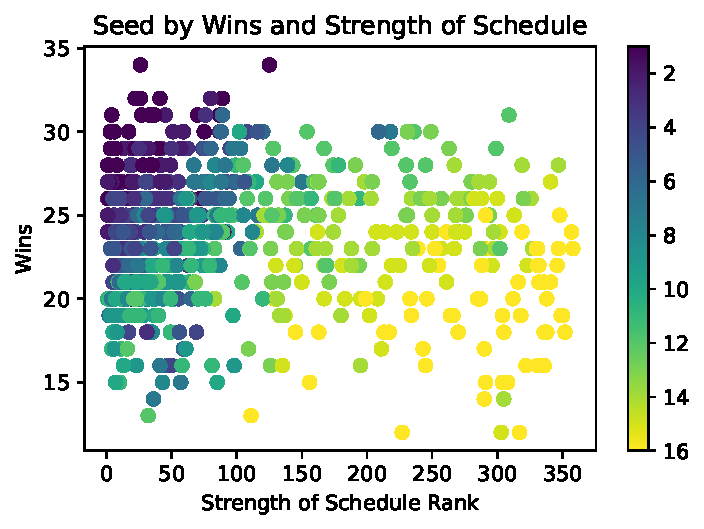
\includegraphics{blog_files/figure-pdf/fig-seed-output-1.pdf}

}

\caption{\label{fig-seed}Scatterplot of Seed determined by Wins and
Strength of Schedule}

\end{figure}

Figure Figure~\ref{fig-map} shows the distribution of March Madness by
states in which the school is located. Texas leads the pack, having a
plethora of schools eligible for March Madness. More of a surprise to
those who are not fans of college basketball, North Carolina ranks
second amongst all states as it has perennial favorites such as Duke and
North Carolina who make the tournament almost every year. The east half
of the US dominates tournament bids outside a few states, namely Texas,
California, and Kansas.

\begin{figure}

{\centering 

\begin{Shaded}
\begin{Highlighting}[]
\ImportTok{import}\NormalTok{ pandas }\ImportTok{as}\NormalTok{ pd}
\ImportTok{import}\NormalTok{ plotly.express }\ImportTok{as}\NormalTok{ px}
\NormalTok{fullstats }\OperatorTok{=}\NormalTok{ pd.read\_csv(}\StringTok{"fullstats.csv"}\NormalTok{)}

\CommentTok{\# Group by state and count the occurrences of each two{-}letter abbreviation}
\NormalTok{state\_counts }\OperatorTok{=}\NormalTok{ fullstats[}\StringTok{\textquotesingle{}State\textquotesingle{}}\NormalTok{].value\_counts().reset\_index(name}\OperatorTok{=}\StringTok{\textquotesingle{}count\textquotesingle{}}\NormalTok{).rename(columns}\OperatorTok{=}\NormalTok{\{}\StringTok{\textquotesingle{}index\textquotesingle{}}\NormalTok{: }\StringTok{\textquotesingle{}state\textquotesingle{}}\NormalTok{\})}

\CommentTok{\# Create a choropleth map}
\NormalTok{fig }\OperatorTok{=}\NormalTok{ px.choropleth(state\_counts, locations}\OperatorTok{=}\StringTok{\textquotesingle{}state\textquotesingle{}}\NormalTok{, locationmode}\OperatorTok{=}\StringTok{\textquotesingle{}USA{-}states\textquotesingle{}}\NormalTok{, color}\OperatorTok{=}\StringTok{\textquotesingle{}count\textquotesingle{}}\NormalTok{, scope}\OperatorTok{=}\StringTok{\textquotesingle{}usa\textquotesingle{}}\NormalTok{, color\_continuous\_scale}\OperatorTok{=}\StringTok{\textquotesingle{}YlOrRd\textquotesingle{}}\NormalTok{)}

\CommentTok{\# Set title and colorbar label}
\NormalTok{fig.update\_layout(title\_text}\OperatorTok{=}\StringTok{\textquotesingle{}March Madness Teams by State\textquotesingle{}}\NormalTok{)}
\NormalTok{fig.update\_coloraxes(colorbar\_title}\OperatorTok{=}\StringTok{\textquotesingle{}\# of Teams\textquotesingle{}}\NormalTok{)}

\CommentTok{\# Show the plot}
\NormalTok{fig.show()}

\CommentTok{\# The field seems to be made up of mainly teams from Texas, California, Virginia, New York, North Carolia and Ohio. The two}
\CommentTok{\# states that stand the most are Texas and North Carolina as Texas features a lot of Power 5 schools, while North Carolina }
\CommentTok{\# is top heavy having perennial favorites such as North Carolina and Duke that make the field almost every year.}
\end{Highlighting}
\end{Shaded}

\begin{figure}

{\centering 

\begin{verbatim}
Unable to display output for mime type(s): text/html
\end{verbatim}

}

\caption{Map of March Madness Teams by State (2012-2022)}

\end{figure}

\begin{figure}

{\centering 

\begin{verbatim}
Unable to display output for mime type(s): text/html
\end{verbatim}

}

\caption{\textbf{?(caption)}}

\end{figure}

}

\caption{\label{fig-map}\textbf{?(caption)}}

\end{figure}

Here's an example of citing a source (see Phillips 1999, 33--35). Be
sure the source information is entered in ``BibTeX'' form in the
\texttt{references.bib} file.

The bibliography will automatically get generated. Any sources you cite
in the document will be included. Other entries in the \texttt{.bib}
file will not be included.

\hypertarget{refs}{}
\begin{CSLReferences}{1}{0}
\leavevmode\vadjust pre{\hypertarget{ref-phil99}{}}%
Phillips, T. P. 1999. {``Possible Influence of the Magnetosphere on
{American} History.''} \emph{J. Oddball Res.} 98: 1000--1003.

\end{CSLReferences}



\end{document}
